\chapter{Introdução}
\label{chap:introducao}

\lipsum[2]

\begin{figure}[h!]
	\centering
	\Caption{Mapa conceitual do estudo da história e relações com o objeto de estudo}
	\label{fig_mapa-5}
	\IBGEtab{}{
	    		\fbox{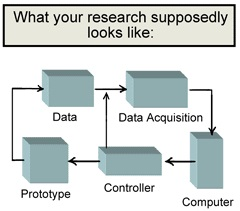
\includegraphics[width=8cm]{figuras/figura-1}}
	}{
		\Fonte{os autores}			
	}	
\end{figure}

\lipsum[2]
\lipsum[2]
\lipsum[2]

%\Gls{latex} e \gls{maths}
\Gls{ambiguidade}
\Gls{braile}
\Gls{coerencia}
\Gls{dialetos}
\Gls{elipse}
\Gls{locucao-adjetiva}
\Gls{modificadores}
\Gls{paronimos}
\Gls{sintese}
\Gls{borboleta}

\begin{figure}[h!]
	\centering
	\Caption{Paradigma segundo processos que caracterizam a EFSFVS como Escola do SUS}
	\label{fig_paradigma}
	\IBGEtab{}{
		
\includegraphics[width=8cm]{figuras/figura-2}
	}{
		\Fonte{os autores}			
	}
\end{figure}

\lipsum[2]
\lipsum[2]

\section{Motivação}
\lipsum[2]
\lipsum[2]

\section{Objetivos}

\lipsum[2]

    \begin{table}[h!]
    	\centering	
    	\Caption{Internal exon scores}
    	\label{tab:internal-3}	
    	\IBGEtab{}{
        	\begin{tabular}{cll}
        		\toprule
        		Ranking & Exon Coverage & Splice Site Support\\
        		\midrule \midrule
        		E1 & Complete coverage by a single transcript & Both splice sites\\
        		E2 & Complete coverage by more than a single transcript & Both splice sites\\
        		E3 & Partial coverage & Both splice sites\\
        		E4 & Partial coverage & One splice site\\
        		E5 & Complete or partial coverage & No splice sites\\
        		E6 & No coverage & No splice sites\\
        		\bottomrule
        	\end{tabular}
    	}{
    		\Fonte{os autores}
    	}
    \end{table}

\lipsum[2]

\subsection{Objetivo Geral}

\lipsum[2]

\subsection{Objetivos Específicos}
	\lipsum[2]
	
	\begin{alineas}
		\item \lipsum[2]
		\item \lipsum[2]
		\begin{alineas}
			\item \lipsum[2]
			\item \lipsum[2]
		\end{alineas}
		\item \lipsum[2]	
	\end{alineas}
	
	\lipsum[2]
	
	\begin{table}[h!]	
		\centering
		\Caption{Fatores de risco intermediários, não ajustados para a mortalidade infantil com malformação congênita, de acordo com as características maternas, Fortaleza, CE, BR, 2001 a 2010}
		\label{tab:internal-1}
		\IBGEtab{}{
    		\begin{tabular}{cll}
    			\hline
    			Ranking & Exon Coverage & Splice Site Support\\
    			\hline
    			E1 & Complete coverage by a single transcript & Both splice sites\\
    			E2 & Complete coverage by more than a single transcript & Both splice sites\\
    			E3 & Partial coverage & Both splice sites\\
    			E4 & Partial coverage & One splice site\\
    			E5 & Complete or partial coverage & No splice sites\\
    			E6 & No coverage & No splice sites\\
    			\hline
    		\end{tabular}
    	}{
			\Fonte{os autores}
		}
	\end{table}
	
\vspace{-1.5em}
\subsubsection{Objetivo Geral}
	\lipsum[2]
%	\cite{lamport1986latex} e \cite{wessberg2000real} e \cite{knuth} e \cite{lamport} e \cite{Maia2011} e \cite{mortalidade}
	
\subsubsection{Objetivo Geral}
	\lipsum[2]
	\acrlong{DATASUS},\acrlong{DNV},\acrlong{DO},\acrlong{ESF},\acrlong{IBGE},\acrlong{MFC},\acrlong{MI},\acrlong{MS},\acrlong{NV},\acrlong{ODM},\acrlong{OI},\acrlong{OMS},\acrlong{ONU},\acrlong{PNI},\acrlong{PSF},\acrlong{RIPSA},\acrlong{RN},\acrlong{SIM},\acrlong{SINASC},\acrlong{SUS},\acrlong{TMI},\acrlong{TMMFC}

\lipsum[2]
	\begin{algorithm}[h!]
		\Entrada{o proprio texto}
		\Saida{como escrever algoritmos com \LaTeX2e }
		\Inicio{
			inicializa\c{c}\~ao\;
			\Repita{fim do texto}{
				leia o atual\;
				\Se{entendeu}{
					vá para o próximo\;
					próximo se torna o atual\;}
				\Senao{volte ao início da seção\;}
			}
		}
		\caption{Exemplo de Algoritmo Versao 3}
	\end{algorithm}
	